\documentclass[tikz,margin=2mm]{standalone}
\pagestyle{empty}

%\usepackage{aistats2020}
\usepackage{amsmath}
\usepackage{bm}
\usetikzlibrary{positioning,calc, arrows}

\begin{document}
	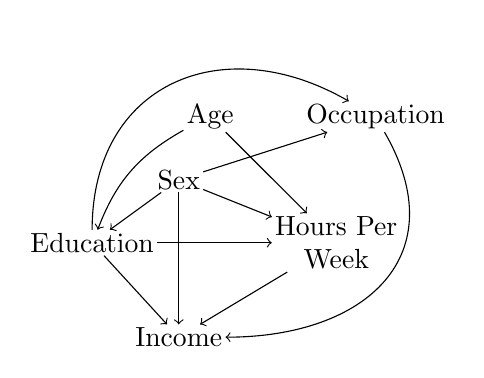
\begin{tikzpicture}
	\begin{scope}[xshift=-2.5cm, yshift=0.7cm]
		\tikzstyle{every node}=[align=center, inner sep=1pt]
		\node (sex) at (-0.7, -0.8) {Sex};
		\node (age) at (-0.3, 0) {Age};
		\node (ed) at (-1.8, -1.6) {Education};
		\node (occ) at (1.8, 0) {Occupation};
		\node (hrpw) at (1.3, -1.6) {Hours Per \\ Week};
		\node (income) at (-0.7, -2.8) {Income};
	
		\draw[->]  (age) to[bend right=20] (ed);
		\draw[->]  (sex) to (ed);
		\draw[->]  (age) to (hrpw);
		\draw[->]  (ed) to (hrpw);
		\draw[->]  (sex) to (hrpw);
		\draw[->]  (ed) to (income);
		\draw[->]  (hrpw) to (income);
		\draw[->]  (occ) to[out=300, in=0, looseness=1.4] (income.east);
		\draw[->]  (sex) to (income);
		\draw[->]  (ed) to[out=90, in=150, looseness=1.3] (occ);
		\draw[->]  (sex) to (occ);	
	\end{scope}
	\end{tikzpicture}

	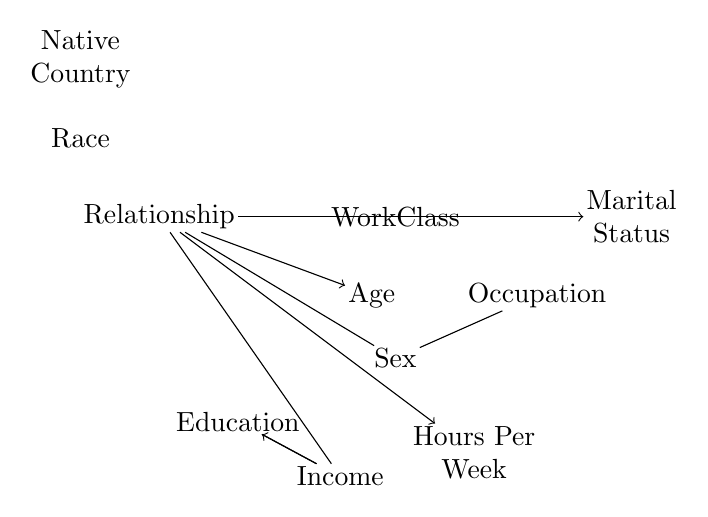
\begin{tikzpicture}
	\begin{scope}[xshift=-2.5cm, yshift=0.7cm]
		\tikzstyle{every node}=[align=center, inner sep=1pt]
		\node (wclass) at (0, 1) {WorkClass};
		\node (sex) at (0, -0.8) {Sex};
		\node (age) at (-0.3, 0) {Age};
		\node (ed) at (-2, -1.6) {Education};
		\node (occ) at (1.8, 0) {Occupation};
		\node (hrpw) at (1, -2) {Hours Per \\ Week};
		\node (income) at (-0.7, -2.3) {Income};
		\node (marital) at (3, 1) {Marital \\ Status};
		\node (reln) at (-3, 1) {Relationship};
		\node (race) at (-4, 2) {Race};
		\node (country) at (-4, 3) {Native \\ Country};

		\draw[] (ed) to (income);
		\draw[] (marital) to (reln);
		\draw[] (occ) to (sex);
		\draw[->] (reln) to (age);
		\draw[->] (reln) to (marital);
		\draw[] (reln) to (sex);
		\draw[->] (reln) to (hrpw);
		\draw[] (reln) to (income);
		\draw[->] (income) to (ed);
	\end{scope}
	\end{tikzpicture}

	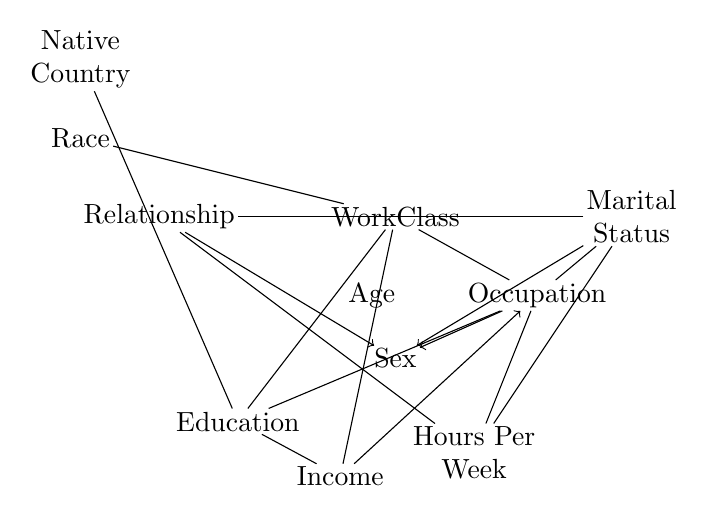
\begin{tikzpicture}
	\begin{scope}[xshift=-2.5cm, yshift=0.7cm]
		\tikzstyle{every node}=[align=center, inner sep=1pt]
		\node (wclass) at (0, 1) {WorkClass};
		\node (sex) at (0, -0.8) {Sex};
		\node (age) at (-0.3, 0) {Age};
		\node (ed) at (-2, -1.6) {Education};
		\node (occ) at (1.8, 0) {Occupation};
		\node (hrpw) at (1, -2) {Hours Per \\ Week};
		\node (income) at (-0.7, -2.3) {Income};
		\node (marital) at (3, 1) {Marital \\ Status};
		\node (reln) at (-3, 1) {Relationship};
		\node (race) at (-4, 2) {Race};
		\node (country) at (-4, 3) {Native \\ Country};

		\draw[]   (wclass) to (ed);
		\draw[]   (wclass) to (occ);
		\draw[]   (wclass) to (race);
		\draw[]   (wclass) to (income);
		\draw[]   (ed) to (occ);
		\draw[]   (ed) to (country);
		\draw[]   (ed) to (income);
		\draw[]   (marital) to (occ);
		\draw[]   (marital) to (reln);
		\draw[->] (marital) to (sex);
		\draw[]   (marital) to (hrpw);
		\draw[->] (occ) to (sex);
		\draw[]   (occ) to (hrpw);
		\draw[->] (reln) to (sex);
		\draw[]   (reln) to (hrpw);
		\draw[->] (income) to (occ);

	\end{scope}
	\end{tikzpicture}

\end{document}
